\chapter{Linear Regression}
\label{chap:linreg}

In regression problems, we take a variable (or multiple variables) as input, and try to fit the output to a continuous expected result function. 



\section{Univariate Linear Regression}
\label{chaplinreg-sect:univar}

In univariate linear regression, we want to predict a single output value $\hat{y}$ from a single input value $x$. Since this is supervised learning, we already have an idea about what the input/output relationship should look like. 



\subsection{The Hypothesis Function}
\label{chaplinreg-sectunivar-subsect:hypfunct}

Imagine we have a problem where the input is $x$ and the output is $y$. In order to do machine learning, there should exist a relationship (a pattern) between the input and output variables. Let's say this function is $y = f\left( x \right)$. In this situation, $f$ is known as the target function. However, this function $f$ is unknown to us, so we need to try and guess what it is. To do that, we form a \textit{hypothesis} function $h\left( x \right)$ that approximates the unknown $f\left( x \right)$. 

For single variable linear regression, our hytothesis function takes two parameters: $\theta_0$ and $\theta_1$. As such, we often write it as $h_\theta\left( x \right)$, and it takes the form
\begin{equation}
\hat{y} = h_\theta\left( x \right) = \theta_0 + \theta_1 x
\end{equation}

Note that this is the equation of a straight line ($y = mx + b$). We're trying to find the values for $\theta_0$ and $\theta_1$ to get our estimated output $\hat{y}$. In other words, we're trying to determine the function $h_\theta$ that maps our input data (the $x$'s) to our output data (the $y$'s). 

Suppose we have the following set of training data:

\begin{center}
\begin{tabular}{c | c}
\textbf{Input } $x$ & \textbf{Output } $y$ \\
\hline
0 & 4 \\
1 & 7 \\
2 & 7 \\
3 & 8 \\
\end{tabular}
\end{center}

We can plot these points, as shown in Figure \ref{fig:linregeg-justpoints}. Let's make a random guess at our hypothesis function: $\theta_0  = 2$ and $\theta_1 = 2$, making our hypothesis function $h_\theta\left( x \right) = 2 + 2x$, as shown in Figure \ref{fig:linregeg-hypotguess1}.

\begin{figure}[h]
	\centering
	\begin{subfigure}[t]{0.45\textwidth}
		\centering
		\graphicspath{{./Figures/}}
		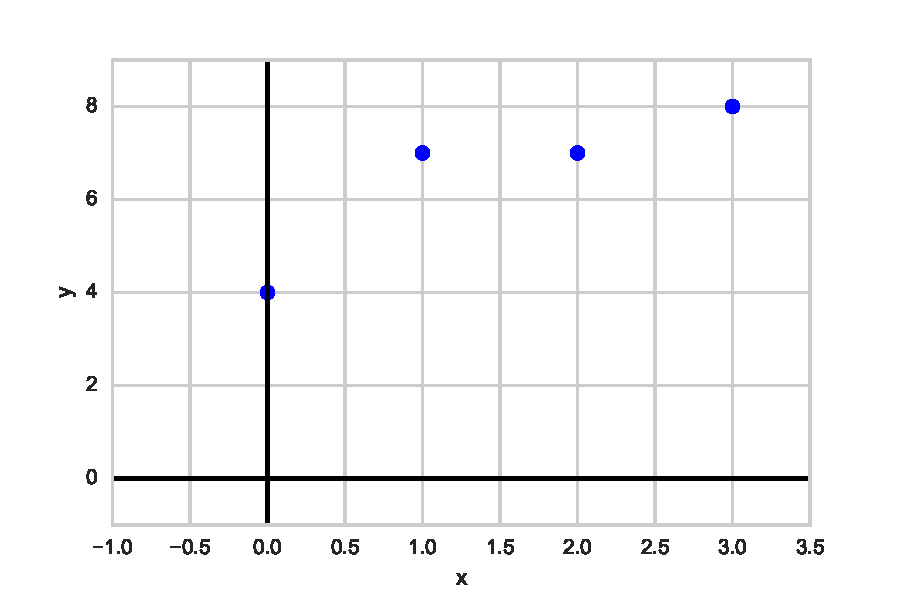
\includegraphics[scale=0.5]{linreg_eg1_plotpoints_noline.pdf}
		\caption{Plotting our example points.}
		\label{fig:linregeg-justpoints}
	\end{subfigure}
	\begin{subfigure}[t]{0.45\textwidth}
		\centering
		\graphicspath{{./Figures/}}
		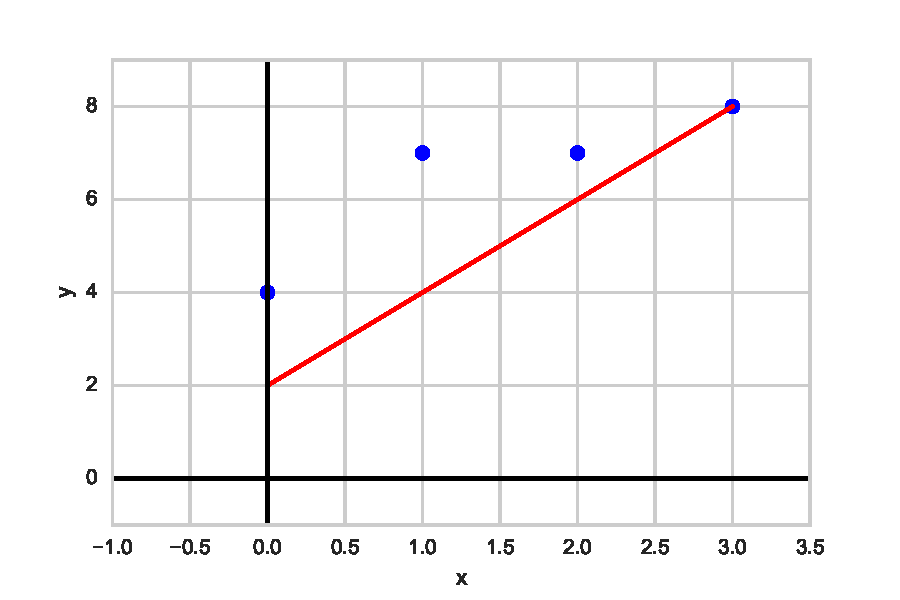
\includegraphics[scale=0.5]{linreg_eg1_plotpoints_line1.pdf}
		\caption{Plotting our example points.}
		\label{fig:linregeg-hypotguess1}
	\end{subfigure}
\end{figure}

Using this hypothesis function for $x = 1$, we have $\hat{y} = h_\theta\left( 1 \right) = 2 + 2 \cdot 1 = 4$. In this case, $\hat{y} = 4$, but $y = 7$, so mabe this isn't the best fit hypothesis.  


\subsection{The Cost Function}
\label{chaplinreg-sectunivar-subsect:costfxn}

The cost function,\footnote{The cost function can also be called the loss function.} is a function used for parameter estimation, where the input to the cost function is some function of the difference between estimated and the true values for an instance of data. In this case, we can use the cost function to measure the accuracy of our hypothesis function. 

The cost function looks at something similar to an average\footnote{It's actually something a bit fancier than a standard average.} of all the results of the hypothesis with inputs from the $x$'s compared to the actual output $y$'s. We define our cost function as follows:

\begin{equation}
J\left( \theta_0, \theta_1 \right) = \frac{1}{2m} \sum_{i=1}^m \left(\hat{y}_i - y_i \right)^2 = \frac{1}{2m} \sum_{i=1}^m \left(h_\theta\left( x_i \right) - y_i \right)^2
\end{equation}

This is known as the \textbf{mean squared error}. If we set $\bar{x}$ equal to the mean of the squares all the $ h_\theta \left( x_i \right) - y_i$, then the cost function is just the mean of $\bar{x}$. The term $\frac{1}{2m}$ is merely a convenience for the computation of gradient descent, which we'll see very shortly. 


\subsection{Gradient Descent}
\label{chaplinreg-sectunivar-subsect:graddsc}

We now have our hypothesis function defined, as well as a way of measuring how well it fits the data. Now, we have to estimate the parameters in the hypothesis function, and that's where gradient descent comes in. 

Let's graph our cost function as a function of the parameter estimates. This can be somewhat confusing, as we are moving up to a higher level of abstraction. We are not graphing $x$ and $y$ itself, but the parameter range of our hypothesis function and the cost resulting from selecting particular sets of parameters. We put $\theta_0$ on the $x$-axis, and $\theta_1$ on the $y$-axis, with the cost function on the vertical $z$-axis.

\begin{figure}[h] %  figure placement: here, top, bottom, or page
   \centering
    \graphicspath{{./Figures/}} %Use this to import an image from a subfolder.
   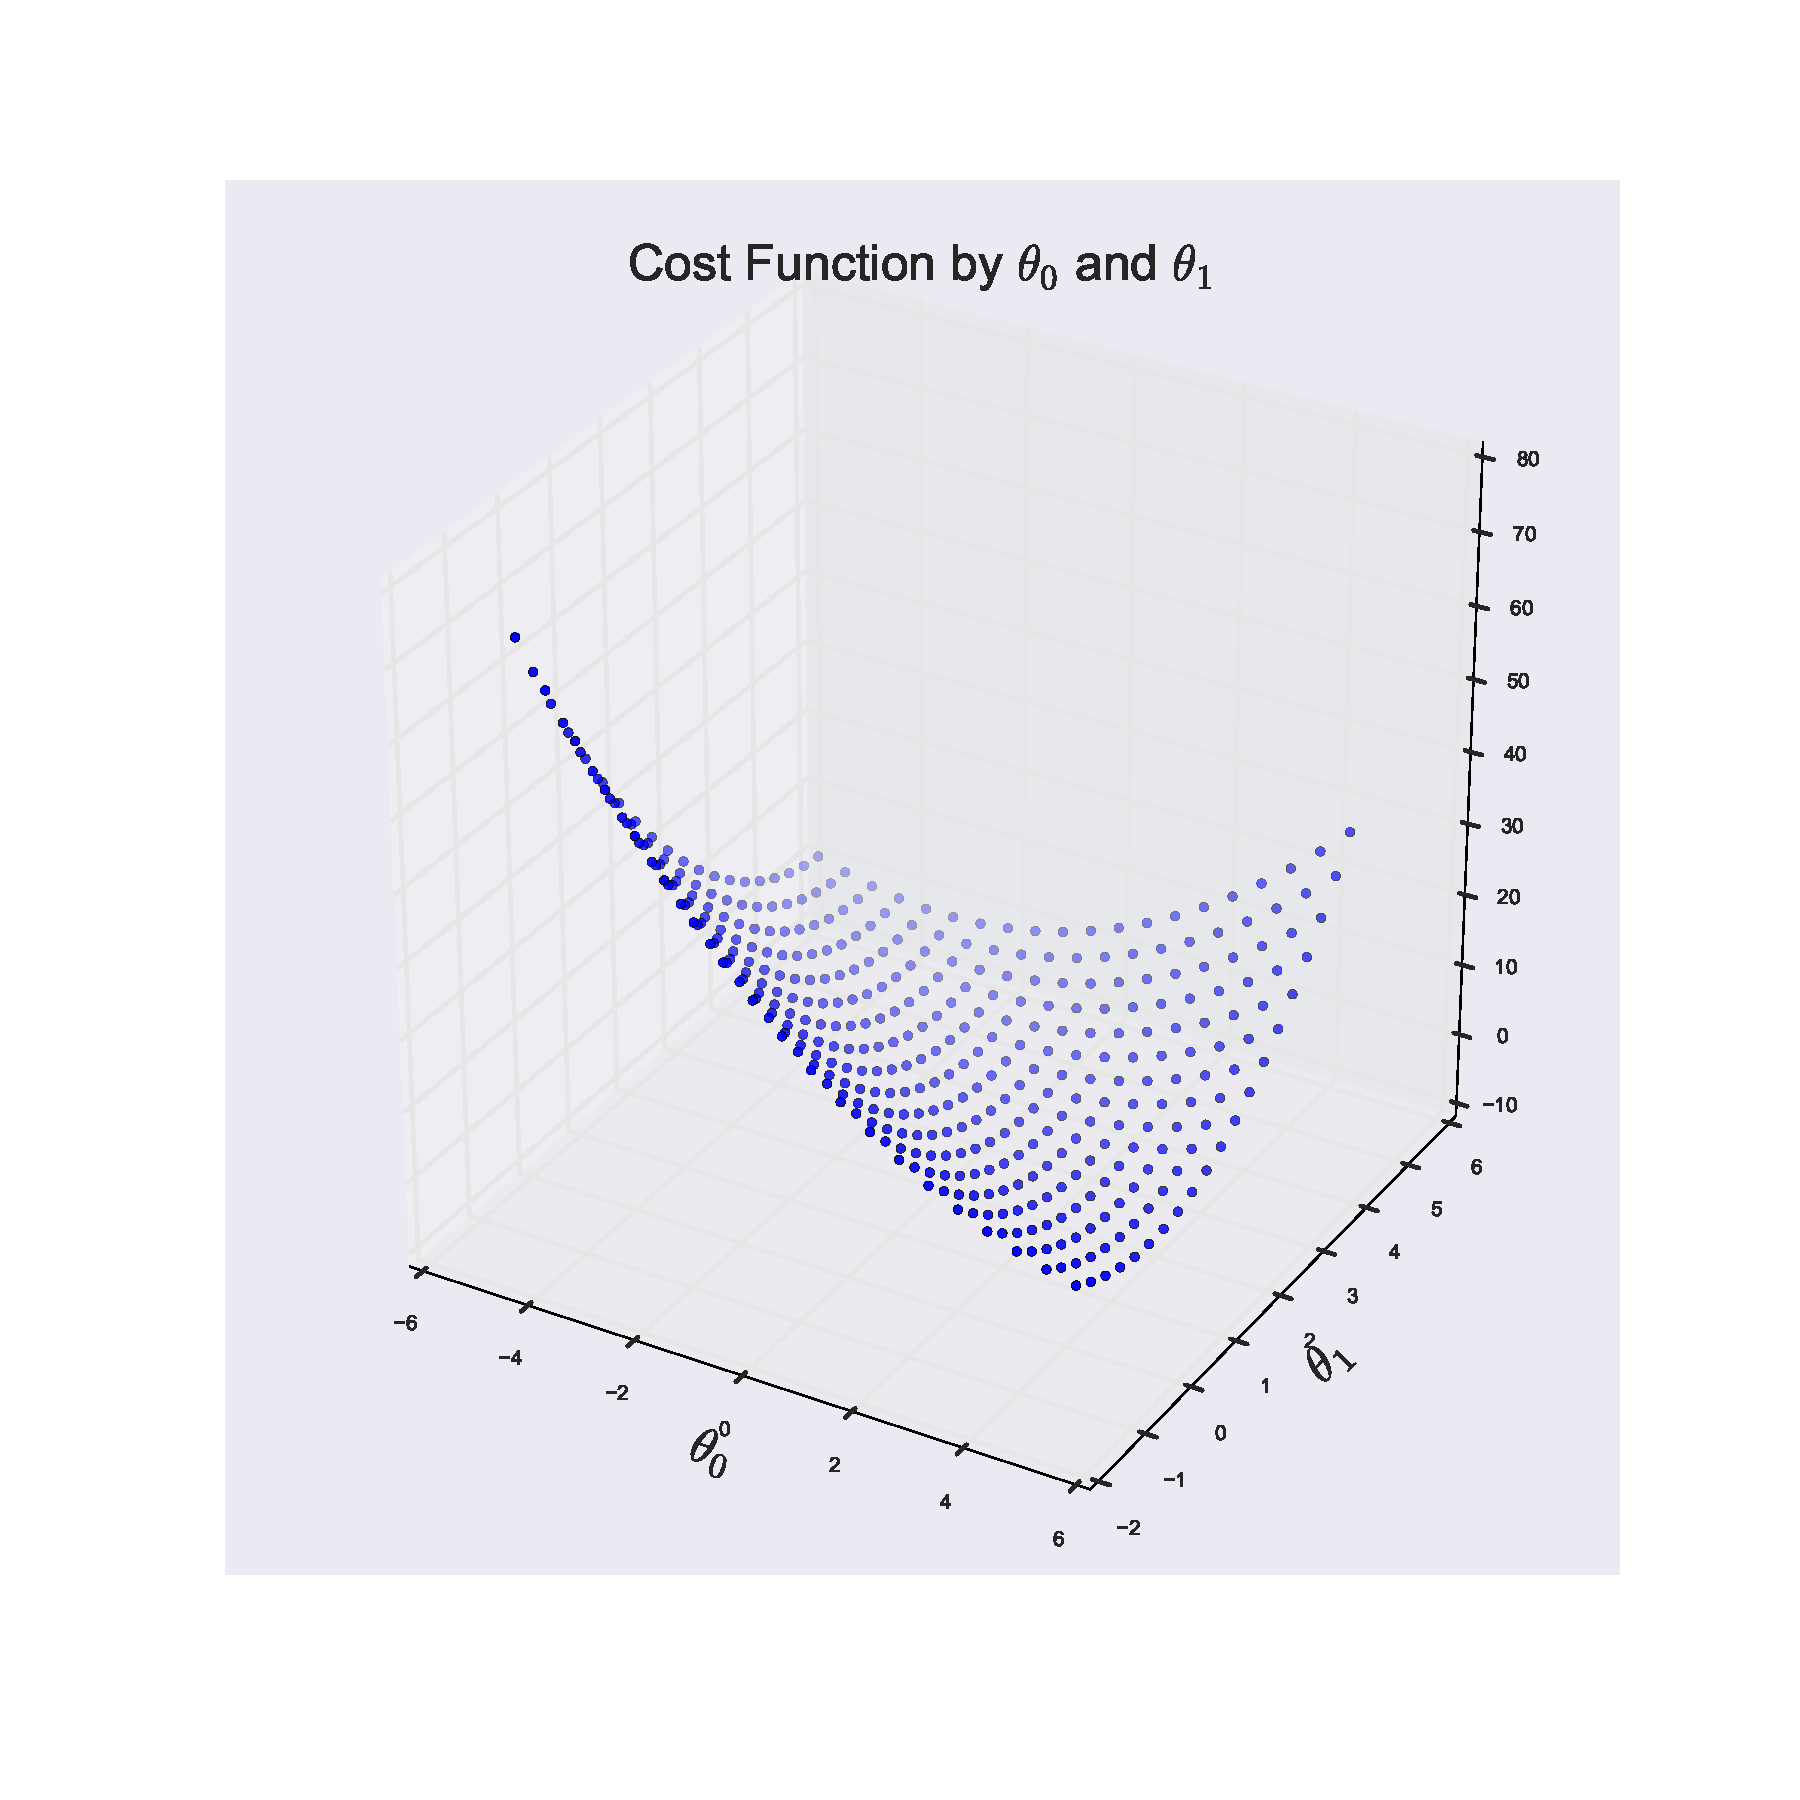
\includegraphics[scale=0.4]{linreg_eg2_cost_func_over_thetas.pdf} 
   \caption[]{Plot of the cost function $J\left(\theta_0, \theta_1 \right)$ using our hypothesis $h_\theta\left( x \right)$.}
   %If using \listoffigures command, then use \caption[short]{long}, where the short caption will appear in the list of figures, and the long caption will appear next to the figure.
   \label{s}
\end{figure}

Our goal is to take the parameters $\theta_0$ and $\theta_1$ for when the cost function is at its minimum. We can calculate this value by taking the derivative of the cost function, which gives us direction of the steepest gradient to move towards. Take a step in that direction, and repeat.The step size is determined by the parameter $\alpha$, which is called the \textbf{learning rate}. The gradient descent algorithm is:

\textbf{Repeat until convergence:}
\begin{equation}
\theta_j := \theta_j - \alpha \frac{\partial}{\partial \theta_j} J\left( \theta_0, \theta_1 \right)
\end{equation}

where $j = 0, 1$ represents the feature index number. 

\subsubsection{Gradient Descent for Linear Regression}
When specifically applied to the case of univariate linear regression, we can derive another form of the gradient descent equation. If we substitute our actual hypothesis function and cost function, we can modify the equation to

\textbf{Repeat until convergence: \{ }
\begin{equation}
\begin{aligned}
\theta_0 &:= \theta_0 - \alpha \frac{1}{m} \sum_{i=1}^m \left( h_\theta\left( x_i \right) - y_i \right) \\
\theta_1 &:= \theta_1 - \alpha \frac{1}{m} \sum_{i=1}^m \left( \left( h_\theta \left( x_i \right) - y_i \right) x_i \right)
\end{aligned}
\end{equation}

\textbf{ \} }

\noindent where $m$ is the size of the training set, $\theta_0$ is a constant that will be changing simultaneously with $\theta_1$, and $x_1$, $y_i$ are values of the given training set. Note that we have separated out the two cases for $\theta_j$ into separate equations for $\theta_0$ and $\theta_1$, and that for $\theta_1$ we are multiplying $x_i$ at the end due to the derivative. 


\section{Multivariate Linear Regression}
\label{chaplinreg-sect:multivarreg}
Let's start by looking at some sample housing data with multiple features. \\

\begin{tabular}{c | c | c | c | c }
Size (feet$^2$) & \# of Bedrooms & \# of Floors & Age (years) & Price (in 1000's of \$) \\ 
$x_1$ & $x_2$ & $x_3$ & $x_4$ & $y$ \\ \hline
2104 & 5 & 1 & 45 & 460 \\
1416 & 3 & 2 & 40 & 232 \\
1534 & 3 & 2 & 30 & 315 \\
852 & 2 & 1 & 36 & 178 \\ 
560 & 1 & 1 & 12 & 155
\end{tabular}

In this, we can introduce some notation:
\begin{itemize*}
\item The variables $x_1$, $x_2$, etc. are the features. 
\item The variable $y$ is the output variable.
\item The number of input features is denoted $n$. In this example, $n = 4$. 
\item $m$ specifies the number of training examples (rows). Here, $m = 5$.
\item $x^{\left( i \right)}$ is the input (features) of the $i^{th}$ training example. So $x^{\left( 2 \right)}$ is the column vector $[1416, 3, 2, 40, 232]$. 
\item $x_j^{\left( i \right)}$ is feature $j$ in the $i^{th}$ training example. Here, $x_1^{\left( 4 \right)} = 852$. 
\end{itemize*}

At this point, we can define the multivariable form of the hypothesis function for linear regression:
\begin{equation}
h_\theta\left( x \right) = \theta_0 + \theta_1 x_1 + \theta_2 x_2 + \theta_3 x_3 + \cdots + \theta_n x_n
\end{equation}

For convenience of notation, we will define $x_0 = 1$ for all feature vectors ($x_0^{\left( i \right)} = 1$). So now, if we include $x_0$, our hypothesis function takes the form:

\begin{equation}
h_\theta\left( x\right) = \sum_{i=0}^n \theta_i x_i
\end{equation}
Now, we can also write the $x$ values and $\theta$ values as vectors:
$$
\vec{x} = \left[ \begin{array}{c}
x_0 \\
x_1 \\
x_2 \\
\vdots \\
x_n
\end{array} \right] \in \mathbb{R}^{n+1} 
~~\mbox{\;\;\;\;\;\;\;\;\;\; and \;\;\;\;\;\;\;\;\;\;}~~
\vec{\theta} = \left[\begin{array}{c}
\theta_0 \\
\theta_1 \\
\theta_2 \\
\vdots \\
\theta_n \end{array}\right] \in \mathbb{R}^{n+1}
$$
In vector notation, this is 
\begin{equation}
h_\theta\left( x \right) = \vec{\theta}^\intercal\vec{x}
\end{equation}
where we transpose $\vec{\theta}$ into a row vector so we're able to take the inner product. 

Now that we have our vector $\vec{\theta} \in \mathbb{R}^{n+1}$, the cost function is
\begin{equation}
J\left(\vec{\theta}\right) = \frac{1}{2m}\sum_{i=1}^m \left( h_\theta\left( x^{\left( i \right)} \right) - y^{\left( i \right)} \right)^2
\end{equation}

\subsection{Gradient Descent for Multiple Variables}
Using our expanded hypothesis and cost functions, the gradient descent algorithm becomes:


\textbf{Repeat until convergence: \{ }
\begin{equation}
\theta_j := \theta_j - \alpha\frac{1}{m} \sum_{i=1}^m \left( h_\theta\left( x^{\left(i\right)} \right) - y^{\left(i\right)} \right) \cdot x_j^{\left( i \right)} ~~\mbox{\;\;\;\;\;\;\;\;\;\; for } j = 0, 1, \cdots, n
\end{equation}
\textbf{ \} }

\subsection{Feature Scaling}
When features are in very different ranges, it can slow down gradient descent dramatically (and also mess up our machine learning algorithms!), because $\theta$ will descend quickly on small ranges and slowly on large ranges, and so will oscillate inefficiently down to the minimum. The way to prevent this is to ensure that all the ranges are roughly the same, ideally:
$$ -1 \leq x \leq 1 $$

Two techniques to accomplish this are \textbf{feature scaling} and \textbf{mean normalization}. Feature scaling involved dividing the input values by the range (max value minus the min value) of the input variable, resulting in a new range of just 1. 

\begin{figure}[h] %  figure placement: here, top, bottom, or page
   \centering
    \graphicspath{{./Figures/}} %Use this to import an image from a subfolder.
   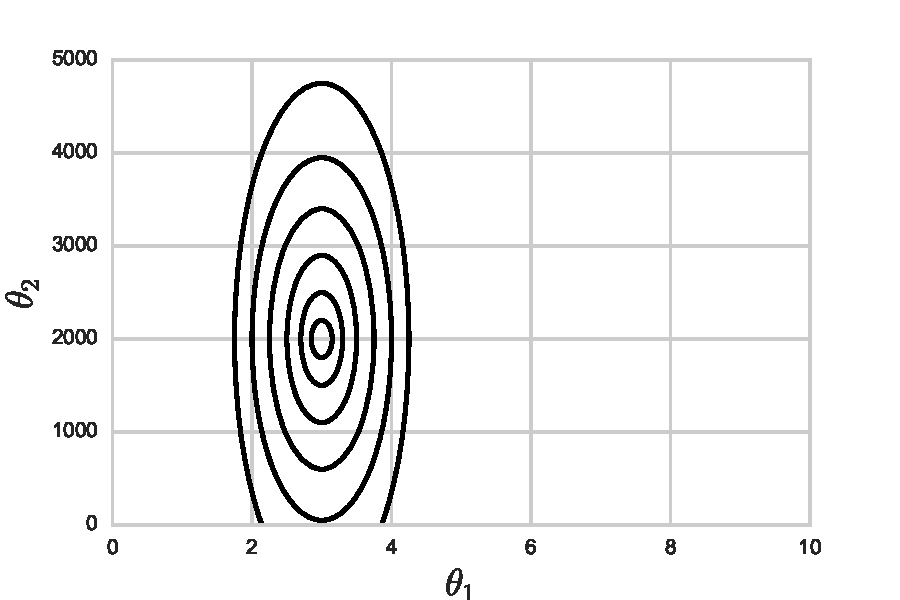
\includegraphics[scale=0.6]{linreg_eg3_why_need_feature_scaling.pdf} 
   \caption[]{When one feature is on a much larger scale than the other, the plot of the cost function will be stretched out in the direction of the larger feature. Here, imagine that $\theta_1$ is the number of bedrooms a house has, and $\theta_2$ is the size in square feet. }
   %If using \listoffigures command, then use \caption[short]{long}, where the short caption will appear in the list of figures, and the long caption will appear next to the figure.
   \label{s}
\end{figure}

Mean normalization involves subtracting the mean value for an input variable from the value for that input variable, resulting in a new mean of zero. To implement both of these simultaneously, use the following formula:
\begin{equation}
x_i := \frac{x_i - \mu_i}{s_i}
\end{equation}
where $\mu_i$ is the average value of $x_i$, and $s_i$ can either be the range ($x_\text{max} - x_\text{min}$) or the standard deviation. 


\subsection{Tips for Gradient Descent}
Here are some of Professor Andrew Ng's tips on implementing gradient descent. 

\begin{enumerate}
\item \textbf{Plot \boldmath$J\left(\theta\right)$.} If you plot $J\left(\theta\right)$ as the ordinate and the number of iterations as the abscissa,\footnote{On a Cartesian coordinate plane, the ordinate is the $y$-axis and the abscissa is the $x$-axis.} the graph should be steadily decreasing with increasing number of iterations. If $J\left(\theta\right)$ ever increases, then $\alpha$ is probably too large. 
\item If $J\left(\theta\right)$ decreases by less then $E$ in one iteration, where $E$ is some very small number, such as $10^{-3}$, then you can declare convergence. 
\item For sufficiently small $\alpha$, $J\left(\theta\right)$ should decrease with every iteration. To choose $\alpha$, try a range of values for $\alpha$ with threefold increases, such as:
$$ \cdots \to 0.001 \to 0.003 \to 0.01 \to 0.03 \to 0.1 \to 0.3 \to 1 \to 3 \to \cdots$$
\item Sometimes, it's better to define new features instead of using the ones given. For example, if we have a house with features frontage\footnote{The width of the land in the front of the house.} and depth,\footnote{The width of the land on the side of the house.} you can combine these into a new feature called area, which is how much land the house sits on.
\end{enumerate}


\subsection{Polynomial Regression}
The form of the hypothesis doesn't necessarily need to be linear of that doesn't fit the data well. We can change the behavior or curve of our hypothesis function by making it quadratic, cubic, square root, or some other form. 

For example, if our hypothesis function is $h_\theta \left(x \right) = \theta_0 + \theta_1 x_1$, we can create additional features based on $x_1$, to get the quadratic function $h_\theta\left(x\right) = \theta_0 + \theta_1 x_1 + \theta_2 x_1^2$, or the cubic function $h_\theta\left(x\right) = \theta_0 + \theta_1 x_1 + \theta_2 x_1^2 + \theta_3 x_1^3$.

When thinking about nonlinear features, it is important to keep in mind that features scaling becomes even more essential than it was for linear regression. If $x_1$ has a range of $1$ to $1000$, the $x_1^2$ has a range of $1$ to $1,000,000$.



\section{Vectorized Equations}
Let's revisit our housing example from \S \ref{chaplinreg-sect:multivarreg}. Recall that we looked at the the following example data, and we'll add an extra column for $x_0$ that always takes a value of one: \\

\begin{tabular}{c | c | c | c | c | c }
{} & Size (feet$^2$) & \# Bedrooms & \# Floors & Age (years) & Price (in \$1000's) \\ 
$x_0$ & $x_1$ & $x_2$ & $x_3$ & $x_4$ & $y$ \\ \hline
1 & 2104 & 5 & 1 & 45 & 460 \\
1 & 1416 & 3 & 2 & 40 & 232 \\
1 & 1534 & 3 & 2 & 30 & 315 \\
1 & 852 & 2 & 1 & 36 & 178 \\ 
1 & 560 & 1 & 1 & 12 & 155
\end{tabular}

From this, we construct a matrix $X$ that contains all of the features from the training data, and a vector $\vec{y}$ of all the output data. 

$$
X = \left[\begin{array}{ccccc}
1 & 2104 & 5 & 1 & 45 \\
1 & 1416 & 3 & 2 & 40 \\
1 & 1534 & 3 & 2 & 30 \\
1 & 852 & 2 & 1 & 36 \\ 
1 & 560 & 1 & 1 & 12
\end{array}\right]
~~\mbox{\;\;\;\;\;\;\;\;\;\; and \;\;\;\;\;\;\;\;\;\;}~~
\vec{y} = \left[\begin{array}{c}
460 \\ 232 \\ 315 \\ 178 \\ 155
\end{array}\right]
$$

Here, $X$ is a $m \times \left(n + 1\right)$ matrix, and $\vec{y}$ is a $m$-dimensional vector. 

Let's go through this again, but this time in full abstraction. Say we have $m$ examples $\left(x^{\left(1\right)}, y^{\left(1\right)}\right),  \left(x^{\left(2\right)}, y^{\left(2\right)}\right), \dots, \left(x^{\left(m\right)}, y^{\left(m\right)}\right)$ and each $x^{\left(i\right)}$ has $n$ features. Then, we have an $\left(n + 1\right)$-dimensional feature vector:

\begin{equation}
x^{\left(i\right)} = \left[\begin{array}{c} x_0^{\left(i\right)} \\ x_1^{\left(i\right)} \\ x_2^{\left(i\right)} \\ \vdots \\ x_n^{\left(i\right)} \end{array}\right] \in \mathbb{R}^{n+1}
\end{equation}

The matrix $X$, which is also called the \textbf{design matrix}, is constructed by taking the transpose of each vector $x^{\left(i\right)}$. Each feature vector $x^{\left(i\right)}$ becomes a row in the design matrix. Just as previously, the output vector $\vec{y}$ is obtained by taking all the labels and stacking them up into an $m$-dimensional vector, and the vector $\vec{\theta}$ is created from stacking all of the parameters for the hypothesis function. 

\begin{equation}
X = \left[\begin{array}{ccccc}
-- & -- & \left(x^{\left(1\right)}\right)^\intercal & -- & -- \\
-- & -- & \left(x^{\left(2\right)}\right)^\intercal & -- & -- \\
-- & -- & \left(x^{\left(3\right)}\right)^\intercal & -- & -- \\
-- & -- & \left(x^{\left(4\right)}\right)^\intercal & -- & -- \\
-- & -- & \vdots & -- & -- \\
-- & -- & \left(x^{\left(m\right)}\right)^\intercal & -- & -- 
\end{array}\right]
~~\mbox{\;\;\;\;\;}~~
\vec{y} = \left[\begin{array}{c} y^{\left(1\right)} \\ y^{\left(2\right)} \\ y^{\left(3\right)} \\ y^{\left(4\right)} \\ \vdots \\ y^{\left(m\right)} \end{array}\right]
~~\mbox{\;\;\;\;\;}~~
\vec{\theta} = \left[\begin{array}{c} \theta_0 \\ \theta_1 \\ \theta_2 \\ \theta_3 \\ \vdots \\ \theta_n \end{array}\right]
\end{equation}

Think back to the start of this section when we separated our table into the design matrix $X$ and the output vector $y$. The design matrix is simply the data as stored in a table put into a matrix. 

In our matrix notation for multivariate regression, the hypothesis function takes the form
\begin{equation}
h_\theta\left(X\right) = X\vec{\theta}
\end{equation}
This will always work since $X$ is an $m\times n$ matrix, and $\vec{\theta}$ is an $n \times 1$ vector. In a similar fashion, the cost function in matrix notation is
\begin{equation}
J\left(\vec{\theta}\right) = \frac{1}{2m} \left(X\vec{\theta} - \vec{y}\right)^\intercal \left(X\vec{\theta} - \vec{y}\right)
\end{equation}

The gradient descent rule can be expressed as
\begin{equation}
\vec{\theta} := \vec{\theta} - \alpha \nabla J\left(\theta\right) 
\end{equation}

There $\nabla$ is the gradient (vector derivative) operator. If we solve this out using our vectorized hypothesis function, we get
\begin{equation}
\vec{\theta} := \vec{\theta} - \frac{\alpha}{m}X^\intercal \left(X\vec{\theta} - \vec{y} \right) 
\end{equation}

\section{The Normal Equation}
The normal equation is a method of solving for the optimal $\theta$ analytically, that is, without iteration. From calculus, if we want to find the minimum of a quadratic equation, we set the derivative equal to zero, and solve. We can apply the same logic to the cost function. If we take the partial derivative $\partial/\partial \theta_j J\left(\theta\right)$ and set this equal to zero for all values of $j$, we'll analytically solve for the minimum. 

The derivation of the normal equation is fairly involved from a linear algebra perspective, so at this point just take it as a fact:
\begin{equation}
\vec{\theta} = \left( X^\intercal X \right) ^{-1} X^\intercal \vec{y}
\end{equation}

When deciding whether to use gradient descent of the normal equation, consider the following:

\begin{tabular}{| l | l |} \hline
\textbf{Gradient Descent} & \textbf{Normal Equation} \\
\hline \hline
Need to choose $\alpha$ & No need to choose $\alpha$ \\ \hline
Needs many iterations & No need to iterate \\ \hline
$O\left( kn^2 \right)$ & $O\left(n^3\right)$, need to calculate $X^\intercal X$ \\ \hline
Works well when $n$ is large & Slow if $n$ is very large \\ \hline
\end{tabular}

With the normal equation, computing the inverse has complexity $O\left( n^3 \right)$. If we have a large number of features, this will cause the normal equation to perform slowly. In practice, when $n$ exceeds $10,000$, it would probably be a good idea to use gradient descent. 

\subsection{Normal Equation Noninvertibility}
When implementing the normal equation, sometimes the matrix $X^\intercal X$ is noninvertible. The common causes are:
\begin{itemize}
\item Redundant features, where two or more features are linearly dependent
\item Too many features (i.e. $m \leq n$). In this case, delete some features or use regularization (which we'll get to later)
\end{itemize}

We typically avoid this problem by coding a pseudoinverse, instead of taking the actual inverse. 

\section{Homework}






















